\twocolumn
\chapter{Synchronous Circuits}
\label{c-Sync}

\section{Feedback}

Memory is formed by a feedback circuit.  The standard way is to take two nand gates or two nor gates and hook their outputs into one of the inputs of the other.

\section{Memory Elements}

SR latches and flip-flops are the fastest, as they are just the latch with possible clocking.  Use them when you need high speed.

\noindent
\begin{tabular}{ll||lp{.25in}ll||ll}
\multicolumn{3}{c}{Characteristic} && \multicolumn{4}{c}{Excitation} \\
S & R & Q && q & Q & S & R \\ \cline{1-3} \cline{5-8}
0 & 0 & q && 0 & 0 & 0 & x \\
0 & 1 & 0 && 0 & 1 & 1 & 0 \\
1 & 0 & 1 && 1 & 0 & 0 & 1 \\
\multicolumn{3}{c}{} && 1 & 1 & x & 0 \\
\end{tabular}

D latches and flip-flops are primarily used in memory applications.  The design process is simple because the simplicity of the excitation table.

\noindent
\begin{tabular}{l||lp{.25in}l||l}
\multicolumn{2}{c}{Characteristic} && \multicolumn{2}{c}{Excitation} \\
D & Q                && Q & D \\ \cline{1-2} \cline{4-5}
0 & 0                && 0 & 0 \\
1 & 1                && 1 & 1 \\
\end{tabular}

T latches and flip-flops are usually used for counters and dividers.

\noindent
\begin{tabular}{l||lp{.25in}ll||l}
\multicolumn{2}{c}{Characteristic} && \multicolumn{3}{c}{Excitation} \\
T & Q                && q & Q & T \\ \cline{1-2} \cline{4-6}
0 & q                && 0 & 0 & 0 \\
1 & q'               && 0 & 1 & 1 \\
\multicolumn{2}{c}{} && 1 & 0 & 1 \\
\multicolumn{2}{c}{} && 1 & 1 & 0 \\
\end{tabular}

JK latches and flip-flops give such easy designs that they are preferred for most every design.  Usually one of the others is only used in the special cases mentioned above.

\noindent
\begin{tabular}{ll||lp{.25in}ll||ll}
\multicolumn{3}{c}{Characteristic} && \multicolumn{4}{c}{Excitation} \\
J & K & Q  && q & Q & J & K \\ \cline{1-3} \cline{5-8}
0 & 0 & q  && 0 & 0 & 0 & x \\
0 & 1 & 0  && 0 & 1 & 1 & x \\
1 & 0 & 1  && 1 & 0 & x & 1 \\
1 & 1 & q' && 1 & 1 & x & 0 \\
\end{tabular}

Typically, the characteristic tables are used when doing analysis, and the excitation table is used for design.

\onecolumn

\section{Counters}



\section{General Design}


Give the logic diagram using any flip-flops you want and a PAL for the state diagram in below.
%    \begin{center}
%    \leavevmode
%    \hbox{%
%    \epsfxsize=3.5in
%    \epsffile{statediag.eps}}
%    \end{center}

    {\color{ans}
    Any undesignated states will go to 111/0, which will be our garbage state.  You could also decide to send it to 000/1, but since this state machine looks for words of the pattern ((01*01*0)*(10*10*1)*)*\footnote{{\color{ans} this is a regular expression that is equivalent to the state machine, regular expressions and their relation to FA/FSM is covered in formal languages and automata theory.  This is included for your information and is thus not expected for you to know for the test.}}, having the undesignated states go to 000/1 would violate the pattern.  Additionally I will use D flip-flops.  I am doing this at home, so I don't have the drawing program, so I will leave the equations for the PAL, the connection is straightforward.

\twocolumn

    \begin{tabular}{c|c||c|c}
      Present &       & Next  &        \\
      State   & Input & State & Output \\ \hline \hline
      000     & 0     & 010   & 1 \\
              & 1     & 100   & 1 \\ \hline
      001     & 0     & 111   & 0 \\
              & 1     & 111   & 0 \\ \hline
      010     & 0     & 011   & 0 \\
              & 1     & 010   & 0 \\ \hline
      011     & 0     & 000   & 0 \\
              & 1     & 011   & 0 \\ \hline
      100     & 0     & 100   & 0 \\
              & 1     & 101   & 0 \\ \hline
      101     & 0     & 101   & 0 \\
              & 1     & 000   & 0 \\ \hline
      110     & 0     & 111   & 0 \\
              & 1     & 111   & 0 \\ \hline
      111     & 0     & 111   & 0 \\
              & 1     & 111   & 0 \\ \hline
    \end{tabular}

    \textbf{Most Significant Bit (S2)}

    \begin{tabular}{c|c|c|c|c|}
    \multicolumn{1}{c}{S0,In$\backslash$S2,S1} & \multicolumn{1}{c}{00} & \multicolumn{1}{c}{01} & \multicolumn{1}{c}{11} & \multicolumn{1}{c}{10} \\ \cline{2-5}
    00 & 0 & 0 & 1 & 1 \\ \cline{2-5}
    01 & 1 & 0 & 1 & 1 \\ \cline{2-5}
    11 & 1 & 0 & 1 & 0 \\ \cline{2-5}
    10 & 1 & 0 & 1 & 1 \\ \cline{2-5}
    \end{tabular}

    \vspace{6pt}

    I will use SOP on the zeros then

    \noindent complement (three encirclements)

    $D2=((S2'\cdot S1)+(S2'\cdot S0'\cdot In')$

    $\qquad +(S2\cdot S1'\cdot S0\cdot In))'$

    \vspace{6pt}


    \textbf{Middle Bit (S1)}

    \begin{tabular}{c|c|c|c|c|}
    \multicolumn{1}{c}{S0,In$\backslash$S2,S1} & \multicolumn{1}{c}{00} & \multicolumn{1}{c}{01} & \multicolumn{1}{c}{11} & \multicolumn{1}{c}{10} \\ \cline{2-5}
    00 & 1 & 1 & 1 & 0 \\ \cline{2-5}
    01 & 0 & 1 & 1 & 0 \\ \cline{2-5}
    11 & 1 & 1 & 1 & 0 \\ \cline{2-5}
    10 & 1 & 0 & 1 & 0 \\ \cline{2-5}
    \end{tabular}

    I will again use SOP on the zeros

    \noindent then complement (three encirclements)

    $D1=((S2\cdot S1')+(S1'\cdot S0'\cdot In)$

    $\qquad +(S2'\cdot S1\cdot S0\cdot In'))'$


    \pagebreak

    \textbf{Least Significant Bit (S0)}

    \begin{tabular}{c|c|c|c|c|}
    \multicolumn{1}{c}{S0,In$\backslash$S2,S1} & \multicolumn{1}{c}{00} & \multicolumn{1}{c}{01} & \multicolumn{1}{c}{11} & \multicolumn{1}{c}{10} \\ \cline{2-5}
    00 & 0 & 1 & 1 & 0 \\ \cline{2-5}
    01 & 0 & 0 & 1 & 1 \\ \cline{2-5}
    11 & 1 & 1 & 1 & 0 \\ \cline{2-5}
    10 & 1 & 0 & 1 & 1 \\ \cline{2-5}
    \end{tabular}

    I will again use SOP on the zeros

    \noindent then complement (five encirclements)

    $D0=((S1'\cdot S0'\cdot In')+(S2'\cdot S1'\cdot S0')$

    $\qquad +(S2'\cdot S0'\cdot In)+(S2'\cdot S1\cdot S0\cdot In')$

    $\qquad +(S2\cdot S1'\cdot S0\cdot In))'$

    \textbf{Output}

    This can be read off the table trivially:

    $Out = S2'\cdot S1'\cdot S0'$
    }
    \onecolumn

\section{State Charts}


\section{ASM Charts}

Large state diagrams get ugly, due to the need to label each input and output, even if they are irrelevant to that state.  Algorithmic State Machine (ASM) Charts take care of this problem, and thus are much easier to read.  Only relevant inputs and asserted signals are listed.

ASM Charts are much like flow charts, and consist of states and decisions connected by directed lines. There are three types of symbols used:
\begin{description}
  \item[rectangle] State block.  The name goes on the upper left (either above or in the box).  The state code goes on the upper right, and the asserted output goes on the lower inside of the box.  Each box is a state, and the system remains in it through a whole clock cycle.
  \item[diamond] Decision block.  The condition goes inside, and the potential answers (usually T/F) goes on the lines exiting the diamond.
  \item[Rounded rectangle] Conditional outputs.  If a Mealy style output is used, then these conditional outputs may be asserted in the conditional output block without changing state.
\end{description}

Basic Rules:
\begin{itemize}
  \item ASMs are deterministic state machines, but they can include parallel conditions, so long as no state is non-deterministic.  Both serial and parallel conditions are performed simultaneously.
  \item Lines must point to a symbol not another line.
  \item At each moment, the system may only be in a state block.  The downstream decision blocks and conditional blocks are calculated during the cycle, so the transition can take place at the clock pulse.
  \item Only state blocks can have multiple inputs.
\end{itemize}

\Example{Bus Arbitrator}

\begin{wrapfigure}{r}{0.35\textwidth}
\vspace*{-.45in}
\begin{center}
\caption{ASM Chart of Bus Arbitrator.}\label{fig-ASM-example}
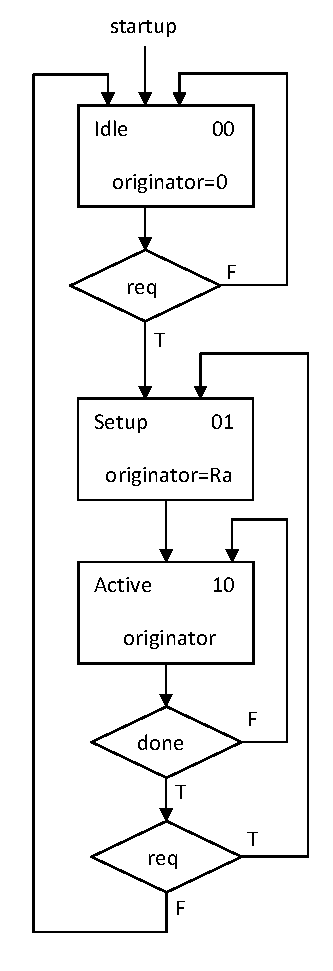
\includegraphics[width=1.9in]{images/ASM.eps}
\end{center}
\end{wrapfigure}

Imagine we are to design a bus arbitrator.  The basic scheme is that there is to be a request line, \emph{req}, that any device can assert as long as it is not currently asserted.  When the request line is asserted, the requestor also puts their identifier on the requestor's address line , \emph{Ra}.  If the system is idle (no one transferring) then the system changes first to a setup state, which sets the originator to the address of the requestor.  When the requestor sees they have the bus, the requestor de-asserts the request line and request address.  The requestor is now the transmitter and we go to the active state.  Since the request lines are free, another device can que a request.  Note only one can que a request as no one else can request once the line is asserted.  When the transmitter is done, the done line is asserted and the request line is checked.  If there is a waiting request this system becomes the transmitter, else the system goes idle.


This is shown in the ASM chart, figure~\ref{fig-ASM-example}.  Let's consider this chart.  We start in the idle state, where the originator is set to zero.  This makes the assumption there is no device with address 0, which is a common assumption.  The alternative is to add a busy line and assert it\footnote{This is inefficient because one extra line is another bit, which could double the number of addresses, then minus one to account for the unused code}.  If no request comes then we stay in idle.  If a request comes we go to setup and copy Ra to originator.  The remote machine must drop the request so we do not list this.  In the remote devices logic when their address gets copied to address, they would switch states and do this.  In any case, the next cycle the system goes to the active state and continues to assert the originator.  When the remote system signals done, the request line is checked.

\clearpage

\section{Block Diagrams}



%\section{Control Flow Graphs}

